% !TeX root = ../../main.tex
\section{Learning the single-cell treatment responses of individual patients} \label{sec:cellot-cohort-iid}
To capture patient-specific drug responses as accurately as possible, we go on to train a \textsc{CellOT} model to learn the responses of each sample to each of their treatment, for a total of 1322 individual models (Figure \ref{fig:iid-prediction}a).
For each model, we train on 75\% of the data and perform model selection and stopping criteria using another 10\%,
and the remaining 15\% of yet unseen control cells to predict their perturbed state using the trained model.

\subsection{Accurately learning treatment responses of melanoma patients}

\begin{figure}[hp!]
  \begin{center}
    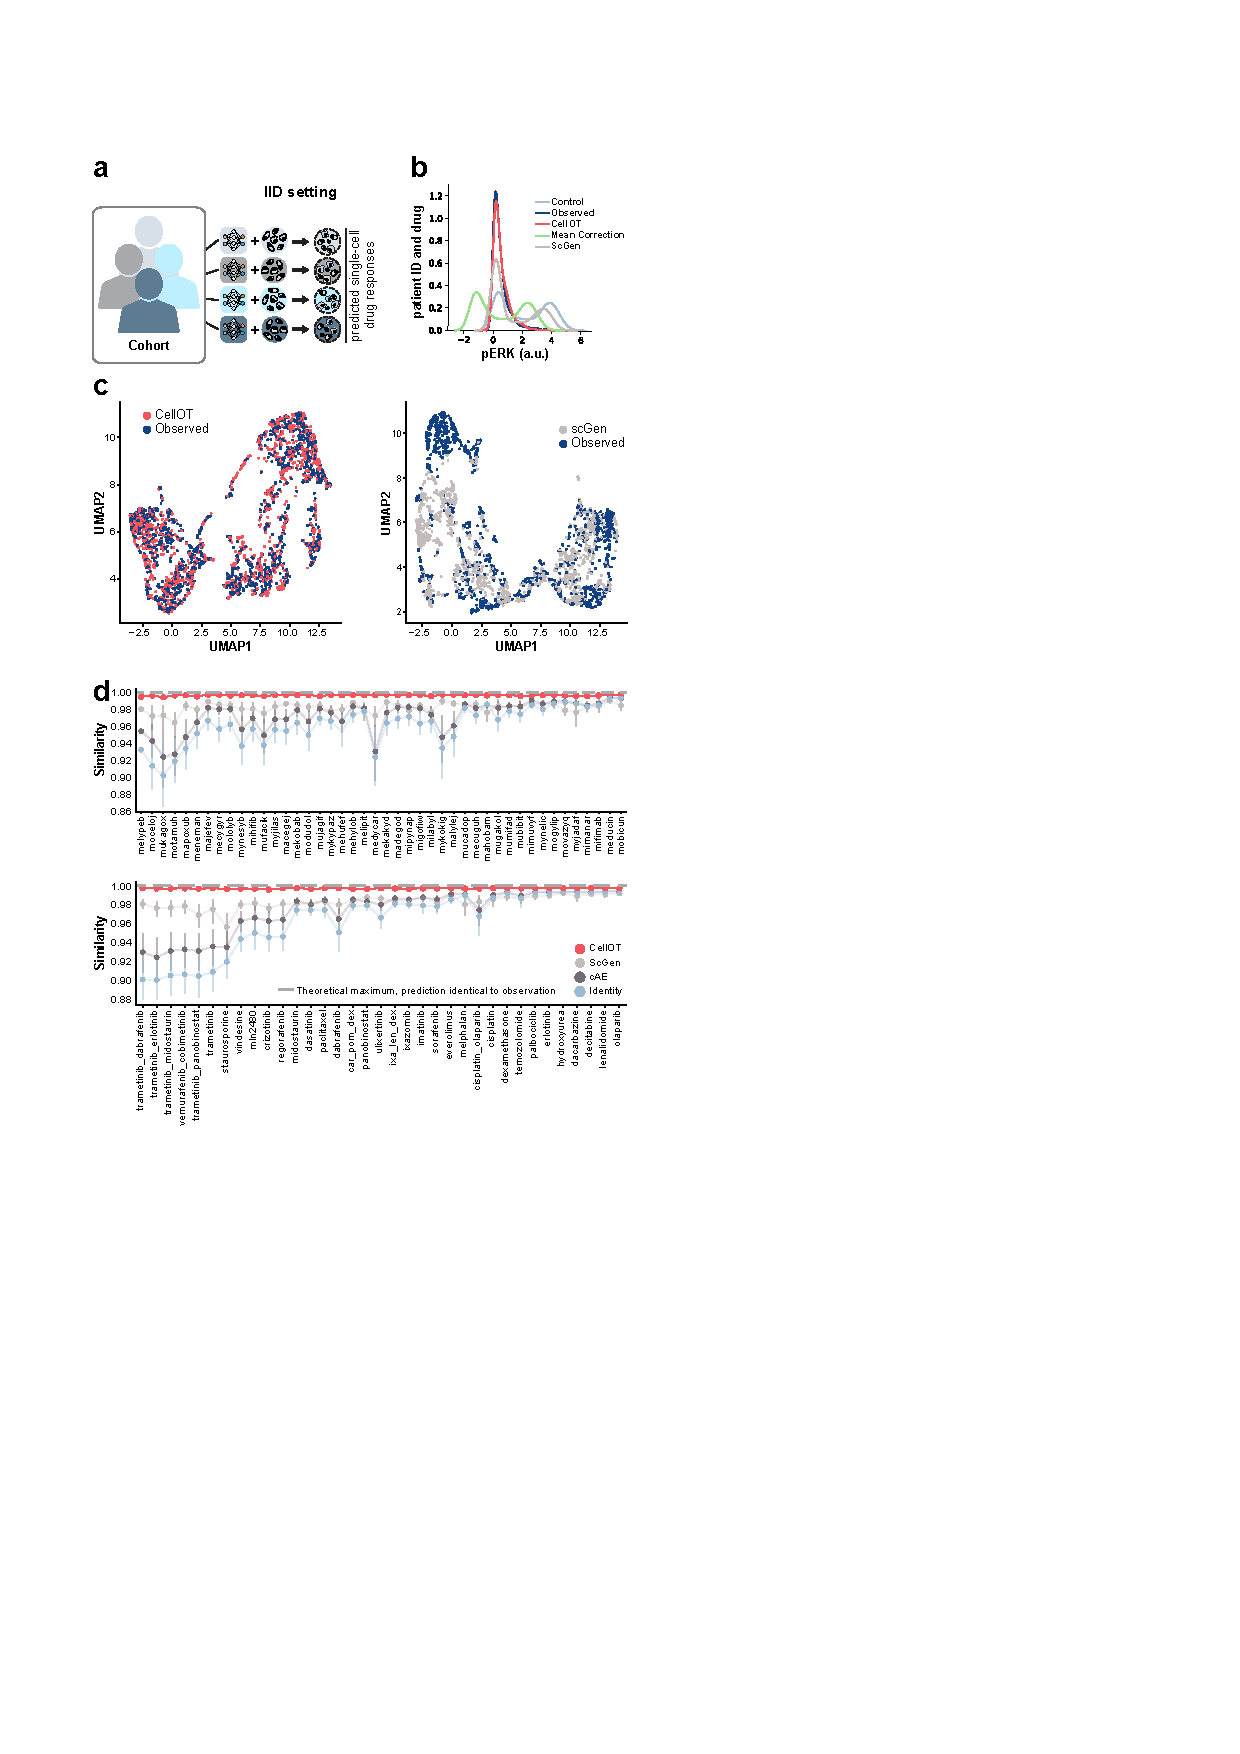
\includegraphics[width=0.5\textwidth]{./figures/cellot-cohort/iid-predictions.pdf}
  \end{center}
  \caption{CellOT learns from and accurately predicts multivariate feature profiles of patient-derived tumor cells treated with cancer drugs.
  a) Graphical representation of the prediction set-up. CellOT is trained on a subset of untreated (control) and drug-treated cells individually for each patient treatment pair. 
  b) Histogram comparing the distribution of predicted-treated pERK single-cell values by CellOT (red), Mean corrections (light green), scGen (grey) to observed-treated values (dark blue) and control (light blue). Unlike other prediction methods, the CellOT-derived marginal almost perfectly overlaps with observed-treated.
  c) Results overview of the methods benchmarking aggregated for samples (top) and drug treatments (bottom). Y axis represents the distributional similarity of  predicted cells to observed cells using an inverse transform MMD metric ($exp^{-MMD}$), where a value of 1 indicates exactness. 
d) UMAPs constructed with equal parts of observed-treated and predicted-treated cells, either by CellOT (left) or scGEN (right).}
  \label{fig:iid-prediction}
\end{figure}

We implement three baseline approaches trained on and predicted with the same data splits as CellOT: a simple model that predicts a homogenous response corresponding to the average response of the sample (mean correction) and two auto-encoder based approaches, \textsc{scGen} \cite{lotfollahi2019} and conditional autoencoders \cite{lopez2018} (cAE), respectively. 

We went on to evaluate model performances both qualitatively and quantitatively by comparing the distribution of predicted cell states to the observed cell states.
We found that across markers and patient treatments, CellOT outperformed the baselines (Figure \ref{fig:iid-prediction}b and Supplementary Figure \ref{fig:cellot-cohort-iid-metrics}).
We also implemented a quantitative framework based on the Earth Mover’s Distance (EMD) \cite{villani2009} and Maximum Mean Discrepancy (MMD) \cite{gretton2012} to measure the similarity of predicted and observed cells in one dimension and multiple dimensions respectively.
For either metric, low values correspond to accurate predictions.
%We went on to compare the implemented baselines to our CellOT predictions using our two metrics and found CellOT-predicted distributional data to be most similar to observed data, and oftentimes hardly distinguishable from the latter (Supplementary Figure \ref{need}).
We summarized our EMD finding both for patients and treatment in relation to the treatment effect and found that CellOT predictions, unlike its comparator baselines, remained accurate even when these were large (Figure \ref{fig:iid-prediction}c).  

Next, we went on to test whether our predictions were not only accurate at the distributional level but also for individual cells.
For this we constructed UMAPs containing equal parts of predicted-perturbed cells and measured-perturbed (observed) cells.
Our hypothesis was that accurately predicted cells would intermix neatly with observed cells.
Indeed, in a UMAP generated with CellOT-predicted and observed cells, we found the whole space to be populated by cells of either origin, indicating that CellOT was capable of predicting indistinguishable perturbation profiles of individual cells.
We found, in contrast, that a UMAP constructed using equal numbers of observed and scGen-predicted cells, displayed areas exclusively populated by cells of one of the two origins, which we believe are caused by inaccurate cell predictions (Figure \ref{fig:iid-prediction}d).
We quantified our observation by implementing a nearest neighbor analysis for which we quantified the identity k=50 neighboring cells for each cell in the original feature space.
Given the equal number of cells from each origin, optimal mixing of the two cell populations would have resulted in a neighborhood value of 0.5. For the displayed treatment, CellOT-Observed achieved a neighborhood value of 0.497 , whereas \textsc{scGen}-Observed was 0.451.
Across all patient-treatment pairs the neighborhood value averaged at 0.495 and 0.477, respectively (Supplementary Figure \ref{fig:cellot-cohort-iid-knn}).
Our quantitative assessment shows that single-cell drug responses of progressed melanoma patients can be predicted accurately using CellOT. 

% TODO: check that all Figure X references are correctly rendered with \ref

Ex-vivo drug profiling has been used successfully to profile cytotoxic effects of various anti-cancer drugs to guide personalized therapy selection, in particular hematological indications \cite{liebers2023, kropivsek2023}.
Different to previous work, the primary aim of the 4iDRP, was to measure the modulation of signaling pathways in response to pharmacological insults with multiplexed readouts.
Our hope at the outset of our study, was that we would identify strong patient-level drug response signatures which would allow us to differentiate between control and treated samples and ultimately use such signatures to derive mechanistic insights about differences in treatment mechanisms and outcomes.  

\begin{figure}[htp!]
  \begin{center}
    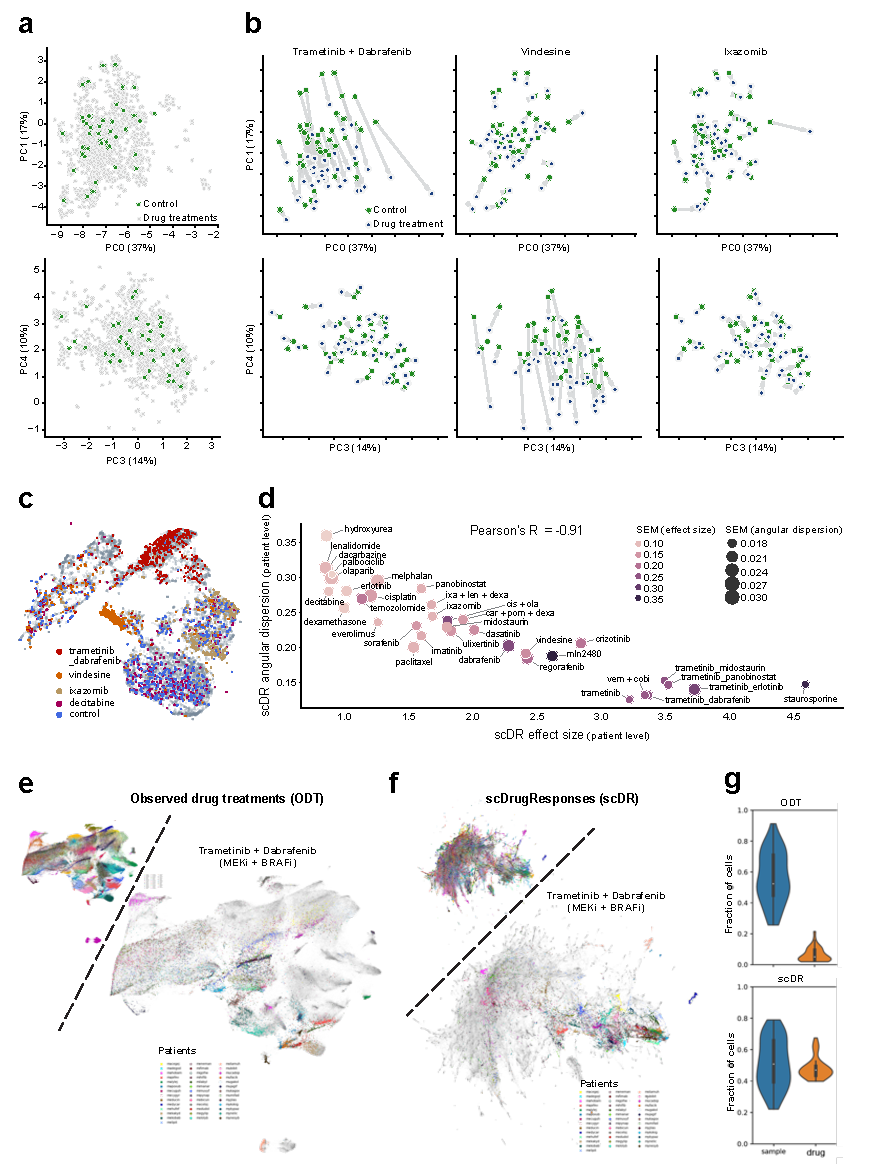
\includegraphics[width=0.5\textwidth]{figures/cellot-cohort/iid-response-structure.pdf}
  \end{center}
  \caption{Unaccounted sample heterogeneity dominates functional measurements of cancer samples. a) Scatter plots of the first 4 PCs of control and average patient response profiles. Green dots represent the average control state of each patient, grey dots the average response each patient takes to a drug.
  b) Scatter plots of the 4 principal components highlighting control and treated patient profiles of three specific treatments. Green dots: patient profiles derived from control cells. blue dots: patient profiles derived from treated cells. Grey arrow: patient-level treatment effect.
  c) UMAP project of control and CellOT-predicted treated cells of a single sample. Dots represent cells and are color-coded by treatment, grey: other treatments.
  d) Scatterplot comparing patient-aggregated single-cell measurements of drug effect size (x axis) and angular dispersion (y axis). Angular dispersion measures the homogeneity of the response, where low values are homogeneous and high values are heterogeneous.
  e) and f) UMAP project of a random selection of observed treated cells (e) and scDRs (f) across all samples and treatments, colored by sample (top). Trametinib - Dabrafenib responses are highlighted in the bottom panels.
  g) Neighborhood analysis in observed drug treated cells (top) and scDRs (bottom). The analysis measures the fraction of cells in the data space neighborhood of each cells sharing either the same sample origin or treatment.
 }
  \label{fig:iid-structure}
\end{figure}

\subsection{Heterogeneity dominates patient drug responses}
To gain an improved understanding of our dataset we first generated aggregated 4i profiles of our patients from control and the corresponding CellOT-predicted-treated cells by averaging single-cell results to patient-treatment profile.
Next, we used the generated profiles to conduct a Principal Component (PC) Analysis and visualized the cohort in two scatter plots using the first and second, and the third and fourth PC, respectively (Figure \ref{fig:iid-structure}a).
We visualized predicted-treated profiles in grey and control profiles in green.
Surprisingly, we find that the control profiles interspersed extensively with predicted-treated profiles.
Further, we found that control profiles were distributed across the first 4 dimensions of our analysis (which represent 78\% of the variability observed) effectively rendering it impossible to distinguish between untreated (control) states of patients of our cohort and the treatments.
This intermixing is consistent with patient-level diversity being a dominant factor of variation across all measurements.

Next, we are interested in understanding to what extent drug treatment effects are distinct and coherent throughout our cohort.
For this, we selected three drug treatments, Trametinib + Dabrafenib (MEK inhibitor + BRAF inhibitor, Tram+Dabra), Vindesine (Vinca alkaloid), and Ixazomib (Proteasome inhibitor), Figure \ref{fig:iid-structure}b.
These treatments were selected as representatives as they each have a different mechanism of action (MOA) and are indicative of the various effects strength measured with our platform.
Thanks to \textsc{CellOT}, we have matched control (green) and predicted-treated profiles (blue), and so we were able to measure and visualize patient-specific drug effects (grey arrow).
 We found that Tram+Dabra indeed affected most samples similarly.
The severity of drug effects, however, varied across the cohort, as indicated by the differing arrow length and heterogeneity in effect size and strength increased in the third and fourth PC.
 Similarly, Vindesine showed a common but variably strong drug effect in the 3rd and 4th PC (Figure \ref{fig:iid-structure}b, second column, bottom row), consistent with the respective PC loadings and MOA of a Vinca Alkaloida \cite{dhyani2022} and variable effects in the first two PCs (Figure \ref{fig:iid-structure}b, second column, top row).
 Unlike the other two highlighted drugs, the Ixazomib showed no consistent drug effect in the visualized PC space at the patient level.  

From these findings, we then explored whether treatment effects could be better described at the single-cell level by potentially overcoming artifacts introduced by a patient-level aggregation approach.
We started by constructing UMAP projects of the control and predicted treated cellular states of a single sample, Figure \ref{fig:iid-structure}d.
Similar to our cohort-level view, we found that both control and predicted-treated cells intermixed heavily.
The control cells formed multiple clusters, akin to cancerous subclones.
For relatively strong perturbations, such as Tram+Dabra and Vindesine, the predicted-treated cells clustered closely together, far removed from their corresponding control cells.
For the less strong Ixazomib perturbation, however, predicted cells formed two distinct clusters, highlighting that within a sample the drug response of cells may very well be heterogeneous and dampen a strong patient-level response.
 %We found similar observations across samples and drug treatments in our cohort (Supplementary Figure \ref{need}).
We investigated the notion further, that cell-to-cell variability in single-cell drug responses may mask patient-level treatment signatures.
To do this we compared treatment effect size and variability in effect direction of single cells for each sample-treatment condition (Figure \ref{fig:iid-structure}e).
We discovered that condition-averaged angular dispersion, a measure of variability in effect direction, was anticorrelated to effect size with a Pearson’s R of -0.91.
and that heterogeneity in effect size, i.e. the extent to which a drug effects cells, increases as the condition-averaged effect size increases (growing diameters along x-axis). 

In total, these findings indicate that to best capture drug responses from a clinically diverse cohort, the poorly defined differences between control and treated states and extensive treatment-dependent single-cell heterogeneity need to be accounted for.
 This requires the quantification of a treatment effect on an individual patient cell as a function of that cell’s untreated (control) state, effectively measuring single-cell drug responses (scDR).
 scDRs can be constructed by subtracting the control state from their corresponding predicted treated state using \textsc{CellOT}.
These scDR are conceptually akin to the drug effect vectors presented Figure \ref{fig:iid-structure}b, however with the key distinction that they represent individual cells and not patient averages.

As a first use-case, we set out to understand whether scDRs or profiles of predicted-treated cells captured treatment effects better, both of which are derived from the same cells .
 For this comparison, we first generated a UMAP containing predicted-perturbed cells from all our patients.
 We found that the observed clusters were dominated by the sample ID, rather than the drug treatment (Figure \ref{fig:iid-structure}e, small UMAP).
 This became particularly apparent when only the cells of individual treatments, e.g. Tram+Dabra were color-coded for their sample ID (Figure \ref{fig:iid-structure}e, large UMAP).
 The UMAP generated with scDRs of the same cells on the other hand, revealed less pronounced sample-dependent clustering (Figure \ref{fig:iid-structure}f, small UMAP) and the Tram+Dabra scDRs clustered primarily in one section of the UMAP (Figure \ref{fig:iid-structure}f, large UMAP).
 To quantify these observations, we performed a nearest neighbor analysis comparable to our approach introduced in Figure \ref{fig:iid-prediction}.
We furthermore find that the neighborhood of predicted-treated cells was heavily enriched for cells from the same sample rather than treatments, whereas for scDRs, neighborhoods were composed of single-cell profiles originating from the same sample and same treatment (Figure \ref{fig:iid-structure}g).

Our findings reveal that extracting consistent cohort-wide drug response profiles from progressed melanoma patient samples is a challenging proposition due primarily to the large differences between the control states of our samples as well as heterogenous drug responses.
 We found that by taking into account both these sources of heterogeneity and generating scDRs, we are capable of capturing relevant biological information describing drug response shared across patient samples. 

\subsection{Informing subcohort behavior from single-cell responses}
\begin{figure}[htp!]
  \begin{center}
    \includegraphics[width=0.65\textwidth]{figures/cellot-cohort/iid-associations.pdf}
  \end{center}
  \caption{
  Single-cell Drug Responses reveal unknown clinical associations and postulated resistance mechanisms.
a) Hierarchical clustering of patient profiles derived from Trametinib + Dabrafenib observed cells (left) and scDR predicted cells (right).
b) Associations of drug responses to clinical features. Total significant associations (left panel, p < 0.05) of scDRs (red) and observed cells (blue). Significant associations based on scDRs (middle panel) and observed cells (right panel). Darker hues indicate more significant associations.
c) Sum of identified clinical associations across all drug treatments for other data modalities.
d) Clinical associations detected using control cell features.
e) and f) Clinical associations detected across three cellular representations and differential responses of relevant driver mutations, Tram+Dabra and BRAF (e) and Paclitaxel and NRAS (f).
}
  \label{fig:iid-associations}
\end{figure}

scDR provide us with access to previously inaccessible representations of cellular processes in patient samples.
Here we show how suitable patient-level descriptors based on scDRs allow for the discovery of differential drug responses that are associated with clinical characteristics of patients.
%We previously introduced MMD as a similarity measurement between two sets of multi-dimensional distributions.
%We extended the concept to perform pairwise patient comparisons of scDR and treated-predicted profiles.

We utilize the MMD metric to compute a patient similarity score over a (subsampled) set of each patient's scDRs.
Then, we performed hierarchical clustering on this patient similarity matrix, generated using either treated or scDR profiles,
and visualized the clinical data associated with each sample as row labels between the dendrogram and the similarity matrix (Figure \ref{fig:iid-associations}a).
As a representative treatment, the Trametinib + Dabrafenib combination is shown, a well know targeted therapy for patients with a BRAF driver mutation.
Here, we found that clustering samples based on observed-treated profiles failed to reveal driver mutation-associated patient groups (Figure \ref{fig:iid-associations}a, left panel).
The clustering of samples using scDRs on the other hand, resulted in patient groups with distinct clinical profiles (Figure \ref{fig:iid-associations}a, right panel).
These results show that a large majority of BRAF V600 mutated samples cluster together, indicative of the targeted nature of the combination therapy.
 Unexpectedly, scDR-based patient profiles revealed further patient groups such as one dominated by samples with NRAS mutations or a third one made up of mostly of samples of ocular subtype.
 This first comparison confirms, that scDRs contain previously inaccessible biological information that links ex-vivo drug responses to clinical patient information.
 Further, this new modality allows for the investigation of differential drug depending on clinical subcohorts. 

We then extended this analysis to all drugs of our 4iDRP platform by developing an algorithm that identifies the overrepresentation of clinical features within a patient group using a hypo-geometric test.
 We found that for all but two drugs, scDRs-based profiles led to the identification of more clinical associations (Figure \ref{fig:iid-associations}b),
 resulting in over 80 known and unknown associations detected by scDR in our dataset (Figure \ref{fig:iid-associations}c).
 Surprisingly, the unperturbed state (control) of tumor cells only revealed differences between samples derived from the brain and other biopsy sites (Figure \ref{fig:iid-associations}d),
 highlighting the differences in tumor biology between brain metastases and metastases of other locations \cite{eichler2011}
 as well as reaffirming the need to compensate for underlying control state heterogeneity in order to accurately measure drug responses.

In line with our qualitative findings for Tram+Dabra, this quantitative approach found associations related to driver mutations and subtypes in scDR profiles but failed to find any significant associations in the observed-treated setting (Figure \ref{fig:iid-associations}b).
 Importantly, patient profiles generated by \textsc{scGen} failed to identify the said associations too.
 We decided to investigate the differential response of BRAF-mutated patients further by comparing their 4iDRP readouts to the rest of the cohort (Figure \ref{fig:iid-associations}e).
 We found 2 4i measurements, pERK and pAKT, to significantly differ between the groups when using scDRs and no significant differences between the two subcohorts in the other two modalities (Control and ODT).
 pERK was reduced in both groups, but showed a stronger reduction in the BRAF-mutated samples, in line with the intended use for patients with a BRAF mutation.
 Intriguingly, the treatment led to a reduction of AKT phosphorylation in the BRAF-mutated samples, whilst it increase levels of pAKT in the other samples.
 This differential response recapitulates extensive findings about a PI3K-mediated escape mechanism in Melanoma \cite{penna2015,irvine2018} and reaffirms the need of a coordinated de-activation of MAPK and MTOR pathways to achieve clinically meaningful treatment responses. 

We, also found unexpected and unreported associations such as a differential treatment response of NRAS-mutated samples to Paclitaxel (Figure \ref{fig:iid-associations}b).
 Paclitaxel is a chemotherapy approved in the early 1990s that induces cell cycle arrest and apoptosis in proliferating cells by preventing depolymerisation of microtubules \cite{panchagnula1998}.
 Fittingly to its MoA, we found upon further investigating of the drug response that NRAS-mutated samples had a reduced Tubulin accumulation compared to the rest of the cohort which was independent of the respective control states and statistically undetectable in the observed-treated measurements (Figure \ref{fig:iid-associations}f).
 This finding points towards attenuated efficiency of Paclitaxel in NRAS-mutated patients, which may serve as the foundation for further experimental and clinical evidence gathering.
 Identifying treatment options which are of particular benefit to patients with NRAS-mutated tumors would be of particular value since NRAS is the second most prevalent genetic alteration in Melanoma (16.4\%), currently lacks targeted therapies and is associated with overall poorer health outcomes \cite{gutierrez-castaneda2020}. 

%Taken together these results show that scDR is more adept at identifying previously known as well as unknown differential drug responses compared against a traditional approach of simply measured treatment effects.
% We further show that the detected differences are often linked to the postulated MoA of the studied drugs, and thus could serve as a hypothesis generator to further refine the use of targeted and chemotherapies to subcohorts of progressed melanoma patients.  

%\begin{figure}[h]
%  \begin{center}
%    \includegraphics[width=0.95\textwidth]{figures/cellot-cohort/ood-eval-logmmd.pdf}
%  \end{center}
%  \caption{
%    Pairwise logMMD differences comparing \textsc{CellOT} and baseline approaches.
%    For each (drug, patient) pair, models are trained on the entire cohort with that patient held out.
%    Each model predicts the drug response of the heldout patient
%    and logMMD values are computed between the distribution of predicted treated states and the true treated states.
%    Negative values correspond to settings where \textsc{CellOT} improves over the corresponding baseline.
%  }
%\label{fig:ood-eval-logmmd}
%\end{figure}
%
%\begin{figure}[h]
%  \begin{center}
%    \includegraphics[width=0.95\textwidth]{figures/cellot-cohort/ood-eval-marker.pdf}
%  \end{center}
%  \caption{
%    Pairwise marker EMD differences comparing \textsc{CellOT} and baseline approaches.
%    For each (drug, patient) pair, models are trained on the entire cohort with that patient held out.
%    Each model predicts the drug response of the heldout patient
%    and marker EMD values are computed between the distribution of predicted treated states and the true treated states.
%    Negative values correspond to settings where \textsc{CellOT} improves over the corresponding baseline.
%  }
%  \label{fig:ood-eval-marker}
%\end{figure}
%
%\begin{figure}
%  \begin{center}
%    \includegraphics[width=0.95\textwidth]{figures/cellot-cohort/ood-predict-marginals.pdf}
%  \end{center}
%  \caption{
%    Predicted response to trametinib dabrafenib combination treatment of each heldout samples.
%    Marginals are shown for the treatment's marker feature, pERK.
%    The inlay shows the selected heldout sample's logMMD score against the rest of the cohort.
%  }\label{fig:ood-predict-marginals}
%\end{figure}
%
%\begin{figure}
%  \begin{center}
%    \includegraphics[width=0.95\textwidth]{figures/cellot-cohort/progression-exclude-mykokig.pdf}
%  \end{center}
%  \caption{
%    Sample mykokig exhibits evidence for low quality cell segmentation and is removed from the progression prediction task.
%  a) Scatter plot of number of treated cells by the variance of intensity features.  Each dot corresponds to a (treatment, sample) pair and treatments of mykokig are shown in blue. Mykokig behaves as an outlier as it has much more cells per treatment than other samples and these cells have low variance in their intensity features.
%  b) Morphology features of mykokig cells indicate the presence of artifacts. The cluster map shows the distribution of each extracted morphology feature (rows) for cells sampled from mykokig and a subset of 5 samples from the full cohort. A large fraction of mykokig cells exhibit a strange unique morphology pattern of small round cells.
%  }\label{fig:progression-exclude-mykokig}
%\end{figure}
%
%\begin{figure}
%  \begin{center}
%    \includegraphics[width=0.95\textwidth]{figures/cellot-cohort/progression-exclude-motamuh.pdf}
%  \end{center}
%  \caption{
%    The predicted responses for sample motamuh are consistently poor and the sample is therefore removed from the progression prediction task.
%    Boxplots show the ranked MMD metric computed between each model's prediction and observed treated states for drugs considered in the progression prediction task.
%    Results for the average model are shown in the IID and OOD setting as well as CellOT predictions in the OOD setting.
%    Sample motamuh consistently ranks worst across all samples in the cohort for these prediction tasks.
%  }\label{fig:progression-exclude-motamuh}
%\end{figure}

\section{Predicting the clinical response of incoming patients}
Accurately predicting the responses of incoming unseen cancer patients is crucial for the optimization of their care.
By anticipating how a patient may respond to different therapies, clinicians can tailor their approach and prepare for potential challenges, enabling proactive interventions and personalized care.
Furthermore, predicting patient response can inform clinical decision-making, resource allocation, and the development of more effective treatment strategies, ultimately improving the overall quality of care delivery for cancer patients.
Here we predict the drug responses of untreated cells from unseen patients.
This is of practical importance, as it forms the foundation for AI-assisted personalized and predictive oncology.
We demonstrate how, from these predictions, we can classify samples into clinically relevant groups, such as the speed of their cancer progression.

\subsection{Predicting treatment effects of unseen patients}
Given observations of how a cohort of patients respond to available treatments, we aim to generalize these responses in order to predict the drug response of an incoming patient.
We refer to these tasks as out-of-distribution, since the cellular states and responses of the test data, i.e. the untreated cells from the unseen patient, are sampled from a different distribution as the training data (the patients in the observed cohort).
Such out-of-distribution tasks are challenging, as we are unable to inform our predictions with the individual effects of the unseen patient.


\begin{figure}[htp!]
  \begin{center}
    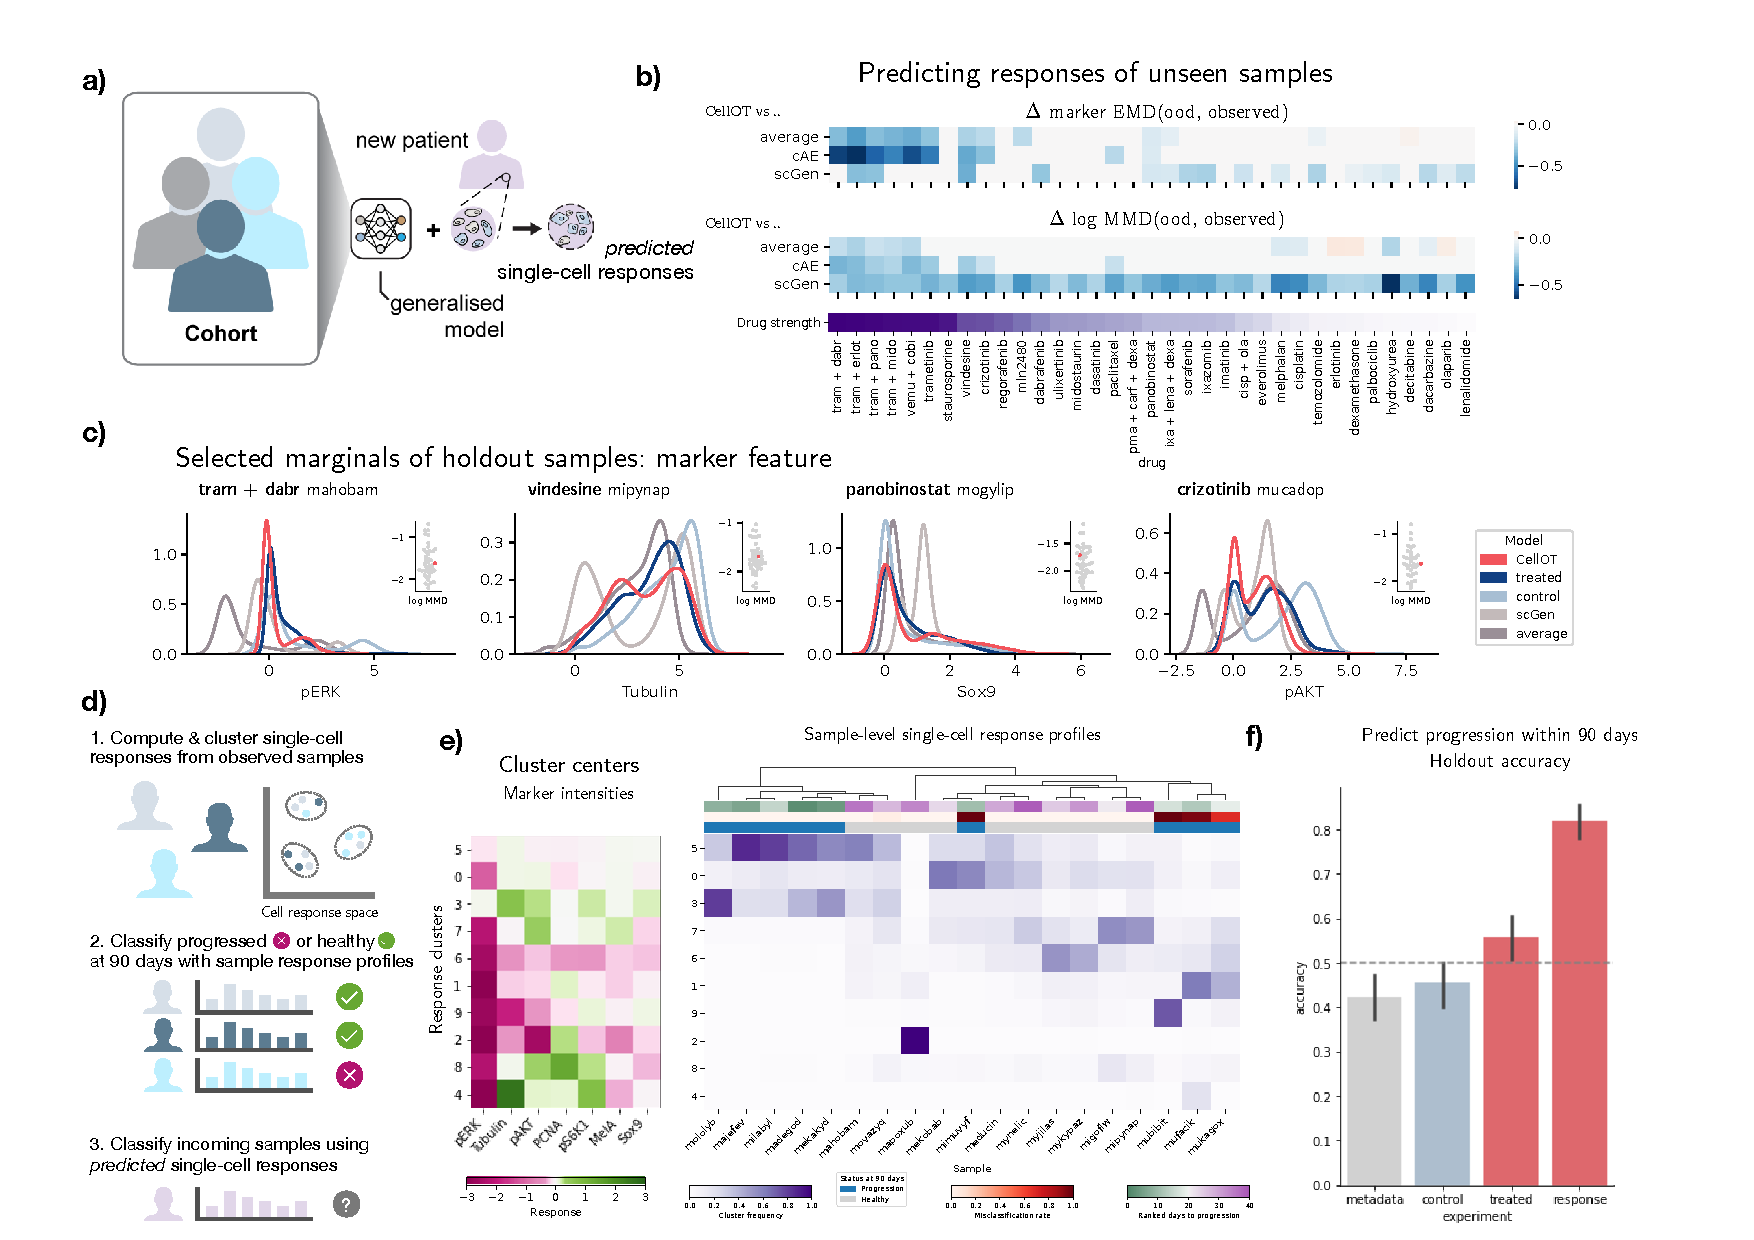
\includegraphics[width=0.95\textwidth]{figures/cellot-cohort/ood.pdf}
  \end{center}
  \caption{
    a) Generalization to heldout samples. For each patient, for each drug, we hold that patient out and train a model on the combined set of observed control and treated cells of the rest of the cohort.
    b) Predictions are made on the held out patient for each (patient, drug, model) triplet and metrics are computed between the responses and predictions of the unseen held out patient.
    We report significant differences (t-test, $p < 0.01$) to each baseline model as colored boxes. Blue hues indicate significant improvements.
    The relative treatment strengths, computed as the metric between the observed control and treated cells, are reported as purple column colors.
    c) Selected predicted marginals of marker features.
    The distribution of CellOT-predicted MMD scores is shown in the inlay, highlighting the selected sample.
    d) Predicting the progression status of incoming samples at 90 days using predicted cellular responses.
    Given access to a training subset of the cohort, IID-predicted cellular responses are clustered and a binary SVM is trained to classify progression status within 90 days using sample level cluster frequencies.
    Incoming samples are predicted using the \emph{OOD}-predicted cellular responses, i.e. without observations of treated states.
    e) kMeans cluster (k=10) centers of marker intensities cellular responses (left) and the cluster frequencies of each sample (right).
    Column colors correspond to the progression label, misclassification rate, and the known days to progression. Samples close to the cutoff are misclassified.
    f) Accuracy to predict progression status within 90 days of incoming samples.
    We compare against similar approaches which represent cells as their predicted treated state, the observed control state, and a random forest on relevant sample metadata.
  }\label{fig:ood-main}
\end{figure}

In order to simulate the clinic environment, we construct, for each patient, a training set composed of all other patients in the cohort (Figure \ref{fig:ood-main}a).
Then, for each perturbation available,
we train a model on the control and treated cells across the whole observed cohort
and apply this model to predict the responses of the unseen patient.
We then evaluate the set of predicted cellular states against the unseen treated cells of the held out patient, as we had done in the iid case.
In addition to the MMD metric \cite{gretton2012}, which considers the state of a multi-dimensional cellular feature set,
we also report the Earth Mover’s Distance (EMD)\cite{villani2009} of the marker feature of each perturbation.
The marker feature is selected by computing the EMD of the observed control and treated states and selecting the feature with the highest average distance,
i.e. the feature that was most affected by the perturbation.
For instance, for Trametinib, this feature is pERK.
The marker feature is of particular interest to the clinician as this typically corresponds to the cellular pathways the treatment is designed to control.

Within each treatment, we compare the ability of CellOT to consistently improve predictions of heldout samples across the whole cohort against baseline approaches.
We first qualitatively compare marker feature distributions of 4 treatments with differing MOAs (Figure \ref{fig:ood-main}c, Supplementary Figure \ref{fig:ood-predict-marginals}) and include the MMD metric corresponding to the selected CellOT predictions, to give a general indication of how well the model is performing (Figure \ref{fig:ood-main}c, dot plot inset).
We find that in most cases CellOT not only outcompetes the baselines in its ability to predict OOD populations, it also reproduces distributional motifs (i.e. subpopulations) observed in the holdout populations.
We then quantitatively compare for which drug treatments does \textsc{CellOT} scDRs consistently outperform other approaches in terms of both MMD and EMD metrics.
This is accomplished with a relative t-test (Figure \ref{fig:ood-main}b, $p < 0.01$) pairwise between metrics computed on \textsc{CellOT} scDRs and other approaches.
The full distributions for the differences of these metrics can be found in Supplemental Figures \ref{fig:ood-eval-logmmd} and \ref{fig:ood-eval-marker}.
We demonstrate that we can make strong gains in many perturbation settings, particularly within the targeted therapies, where treatment effects tend to be quite strong.
Other treatments with more subtle effects, are more difficult to generalize as these perturbations tend to be more subtle and sample-specific effects may become as dominant as the drug effect.
Here, \textsc{CellOT} rarely underperforms against the baselines, and in the few cases when it does, treatment effect sizes are small such as for Olaparib.
We believe these effects are explained by the size of our cohort, which is currently quite large, but may not be large enough to learn to generalize such nuanced responses.
Note that while \textsc{scGen} tends to capture the response of a particular marker feature (EMD), it struggles to capture realistic cellular states (MMD), while the other baseline methods have the inverse behavior.
\textsc{CellOT} typically is able to offer the best of both, highlighting both its accuracy and robustness.

%Within each treatment, we compare the ability of CellOT to consistently improve predictions of heldout samples across the whole cohort against baseline approaches.
%Figure \ref{fig:ood-main}b shows for which treatments there are significant differences across the whole cohort between
%the metric reported by CellOT and the baseline approach, as measured by a relative t-test (p-value < 0.01).
%The full distributions for the differences of these metrics can be found in Supplementary Figures \ref{fig:ood-eval-logmmd} and \ref{fig:ood-eval-marker}.
%We demonstrate that we are able to make strong gains in many perturbation settings, including most of the targeted therapies.
%These therapies are of particular interest as they are among some of the most commonly administered treatments \cite{need} and, in addition, tend to have the strongest effects.
%Many other treatments tend to have more subtle effects, wherein individual effects can dominate the response and thus generalization is difficult to attain.
%However, CellOT rarely underperforms against the baselines, and in the few cases when it does, it does so with small effect sizes.
%Note that while \textsc{scGen} tends to capture the response of a particular marker feature (EMD metric), it struggles to capture realistic cellular states (MMD metric), while the other baseline methods have the inverse behavior.
%CellOT is able to offer the best of both, highlighting its robustness and stability.
%We furthermore provide some example marginals (Figure \ref{fig:ood-main}c, full set in Figure \ref{fig:ood-predict-marginals}), showcasing how CellOT is able to learn biologically relevant states.
%We include the MMD metric corresponding to the selected CellOT predictions, to give a general indication of how well the model is performing.

\subsection{Identifying at-risk patients from predicted cellular responses}
Finally, we demonstrate clinical utility of the predicted drug responses of holdout samples by training a model to predict binarized time to progression (TTP) of patients at 90 days.
The ability to predict and understand progression is clinically relevant, as it indicates cancer aggressiveness \cite{porreca2024} and allows clinicians to individualize the screening schedule of at-risk patients.
In this experiment we demonstrate how scDRs to clinically relevant treatments, selected on a case-by-case basis from a board of medical professionals, can be used to discriminate between samples from patients who progress quickly and those who do not.
To achieve our goal, we construct patient representations of our training set and hold-out sample.
 We then train a Support Vector Machine (SVM) on the training set representation to discriminate between samples of patients with disease progression before 90 days.
 Next, we use the trained SVM and the representation of the hold-out sample to assign the respective patient to the correct progression class (Figure \ref{fig:ood-main}d).
 We generate our patient representations by first creating response signatures with Kmeans clustering of scDRs from sample-treatment pairs (as in Figure \ref{fig:iid-prediction}) and describe the molecular characteristics of these signatures with the average of each 4i features (Figure \ref{fig:ood-main}e).
 We then produce the test set patient representations by computing the relative fraction of cells of each sample assigned to the response signatures. To represent holdout patients, we use the same routine but use OOD scDRs (Figure \ref{fig:ood-main}e).
 Note that while the clustering and patient representations are done only on each training set, Figure \ref{fig:ood-main}e are computed on all samples for the sake of visualization.
 
To ensure that we select treatments that are relevant to the situation of individual patients, we limit ourselves to the treatments that had been prescribed to samples by the medical board associated with the Tumor Profiler project.
From the total cohort, 22 samples had been prescribed a studied small molecule treatment.
Of these 22, we removed three samples due to quality control: \textsc{mykokig}, had evidence of unfiltered artifacts in its observed treated cells (Supplmental Figure \ref{fig:progression-exclude-mykokig}), \textsc{motamuh}, as it represents an extreme outlier in IID and OOD response prediction tasks (Supplemental Figure \ref{fig:progression-exclude-motamuh}), and \textsc{mecygyr}, as it had showed evidence of immediate progression at the start of the study ( $< 5$ days), leaving a subcohort of 19 samples.
Of these 19, 9 progress within 90 days and 10 do not, which yields a balanced binary prediction task.
We simulate the clinic environment by splitting the patients into a train (75\%) and test (25\%) set, (i.e. within each split, 4 of the 19 samples are heldout), where we have access to the control and treated cells of all patients in the training set, and can only access the control cells of patients in the testset.

Our prediction model, summarized in Figure \ref{fig:ood-main}d, works as follows: first, single-cell responses are clustered and patients are represented as frequencies over these clusters, and then an SVM classification model is trained to predict the binary progression status using the patient representations.
To construct the patient representations of the training set, a KMeans clustering is computed using the single-cell treatment responses from all patients in the training set, as predicted using the IID \textsc{CellOT} models, described in section \ref{sec:cellot-cohort-iid}.
We perform a soft assignment of each cell to the $k$ cluster centers, via a softmax transformation over the negative distances to each cluster center, to smooth cluster assignments and help include a notion of cluster similarities, Figure \ref{fig:ood-main}e left.
After this step, each cell is now represented as a probability over the set of cluster centers, Figure \ref{fig:ood-main}e right.
A patient-level representation is constructed by averaging the cluster assignments over all cells from each patient.
At test time, the OOD-predicted cell responses are used instead of the IID, as we are unable to access their treated cell states.
The predicted responses are mapped to the cluster centers, the sample frequencies are computed and the held out sample is classified with the SVM.
Note that the visualizations in Figure \ref{fig:ood-main}e are constructed on IID responses of all samples in the subcohort.
Within each split, these structures are re-computed on the training set only.

Since this is a balanced classification task, we report accuracy as our metric and consider 50\% a trivial lower bound.
For each model setting we perform 100 75\%-25\% train-test splits, i.e. in each split, 4 of the 19 samples are heldout.
We include a model that predicts the progression stats at 90 days with meta information at the sample level, specifically a random forest over the subtype, lines of treatment, and known driver mutation, represented as the concatenation over one-hot encodings of each category.
We furthermore compare our approach to a similar approach that uses predicted treated states, control cells, and single-cell responses predicted by baselines.

The prediction accuracy of holdout samples over 100 train-test splits are shown in Figure \ref{fig:ood-main}f, where we compare using single-cell responses to using control and (predicted) treated states.
In addition, we include a random forest model trained on relevant metadata information, the sample’s subtype, known driver mutation and lines of treatment.
The random forest trained on sample metadata and SVM classification using control states only struggle to perform, yielding accuracies of 0.478 (95\% confidence interval of 0.395 and 0.500).
The SVM classification using treated states fares slightly better, reporting accuracies of 0.558 (95\% c.i. of 0.505 and 0.613).
We see the most drastic improvement using \emph{response} information, which reports accuracies of 0.820 (95\% c.i. of 0.783 and 0.826).
Comparisons to the autoencoder approaches as well as ablations over the number of clusters can be found in  Supplemental Figure \ref{fig:survival-accuracies}, where we show specifically that \textsc{CellOT} responses are stable with respect to classification parameters and out perform baseline approaches.

A benefit of using a straight-forward clustering approach is the ability to interpret the behavior of the model.
We can interpret the decisions made by the model by analyzing the cluster means and patient frequencies over them shown in Figure \ref{fig:ood-main}e.
Here, progression status at 90 days and the misclassification rate of test set samples are shown as row colors.
We see that cells from cluster 5 exhibit a general non-response to the selected perturbations.
Furthermore, samples that have high representation of these responses are more likely to progress,
while samples that exhibit higher degrees of heterogeneity in response are shown to have a better progression status.


\subsection{Learning differential responses with conditional parameters}

\begin{figure}[htp!]
  \begin{center}
    \includegraphics[width=\textwidth]{figures/cellot-cohort/condot.pdf}
  \end{center}
  \caption{
    Predicting strongly differential responses to Dabrafenib of holdout samples using Conditional CellOT.
    a) Dendrogram of sample-level pairwise similarities of Dabrafenib responses, computed using the MMD distances between each sample's distribution of IID-predicted responses reveal similarly responding clusters of non-BRAF samples, BRAF samples with no lines of treatment, and BRAF samples with at least one line of treatment.
    Samples (columns) are colored based on the number of lines of treatment and driver mutation status.
    b) Differential effect strength of Dabrafenib, measured using the EMD of its marker, pERK, between control and treated cells of samples with and without the BRAF driver mutation that the treatment targets.
    c) Predicted responses of pERK for samples with and without the BRAF driver mutation, in both IID and OOD settings.
    OOD \textsc{CellOT} is not able to generalize the differential responses out-of-distribution, while the conditional model has improved performance when compared to the IID model.
    d) Improvements of the pERK marker EMD for predictions made by the conditional CellOT vs other approaches. The metric is computed on the predictions of each approach on cells from holdout samples and the pairwise differences to conditional CellOT are shown. Negative values correspond to improvements Conditional CellOT makes. 
    e) pERK marker marginals for CellOT and conditional CellOT models for BRAF positive (top) and negative (bottom) samples.
  }\label{fig:conditional-ot}
\end{figure}

A common strategy in the design of cancer therapies is to tailor the treatment to interact with some specific mechanism that fails across a number of different cancers.
These \emph{targeted} therapies would, for instance, be designed to treat patients with some driver mutation, such as the infamous BRAF driver mutation.
In such cases, the cellular profile might not capture information crucial to determining the nature of the response, e.g. the presence of the BRAF mutation,
and therefore \textsc{CellOT} performance, as we have described thus far, may struggle.
Here include sample metadata in the inputs of \textsc{CellOT}, by way of \emph{conditional} parameters, in order to help the transport function learn such differential responses.

Here, we focus on the dabrafenib treatment, a targeted therapy to treat BRAF-positive patients.
We observe a strongly differential structure in the responses across the cohort.
Sample similarities are determined by computing the MMD between the learned (IID) single-cell responses of each pair of samples.
Figure \ref{fig:conditional-ot}a shows a dendrogram computed over the set of these pairwise similarities where were we find three main clusters: non-BRAF samples, BRAF positive samples with no previous lines of treatment, and BRAF positive samples with at least one line of treatment.
While the differential response across BRAF status can be easily explained by the targeted nature of the treatment, the differential response to number of treatment lines might be due to a particularly advanced or difficult cancer that necessitates several rounds of treatment.
Figure \ref{fig:conditional-ot}b shows the differential response of pERK, the marker feature for dabrafenib, across BRAF mutation status, by computing the EMD of pERK between the control and observed dabrafenib responses.
Here we observe that dabrafenib induces a strong pERK response in patients with the BRAF mutation, but a weak response in those without,
an observation is in agreement with the intended design and use of the drug.

In order to learn the strongly differential response of dabrafenib,
we train a version of CellOT whose inputs inputs are \emph{conditioned} \cite{bunne2022} with the status of the sample's driver mutation and lines of treatment. 
These conditional parameters are able to inform and influence its learned responses with clinical metadata
This is achieved by concatenating a one-hot encoding of each metadata to the cellular features.
Note that while the potentials trained by \textsc{CellOT} must be convex in their inputs,
they do not need to be convex in these conditional inputs \cite{amos2017}.

By comparing the conditional \textsc{CellOT} predictions to vanilla \textsc{CellOT} trained in the IID and OOD settings, we observe that the conditional version is able to better capture the differential pERK responses.
In Figure \ref{fig:conditional-ot}c) we see that the IID \textsc{CellOT}, which is able to learn patient-specific responses, indicates that BRAF samples respond to dabrafenib by decreasing pERK levels, while non-BRAF samples have a negligible response.
OOD \textsc{CellOT}, on the other hand, predicts all samples, regardless of their BRAF status, to respond to dabrafenib with a slight decrease of pERK levels, and report little to no difference across BRAF status.
The conditional \textsc{CellOT}, however, is able to correctly predict a differential response across BRAF status.
This is further quantified in Figure \ref{fig:conditional-ot}d), where we see consistent improvement in OOD pERK prediction when using conditional \textsc{CellOT} over vanilla \textsc{CellOT} and other baseline models.
Finally, marginals highlighting the learned differential responses are shown in Figure \ref{fig:conditional-ot}e,
where it can been seen that conditional \textsc{CellOT} indeed learns the pERK response of BRAF positive samples (top) and non-response of negative (bottom).
